\part{Visualizations}

% ------------------------------------------------------------
% ------------------------------------------------------------
\section{Data Set}
\begin{frame}[allowframebreaks, fragile]
\frametitle{Data Set for Tutorial}
	Data set for this tutorial comes from State of California.  Please export it to CSV from: \\
	\vspace{5pt}

	\noindent \url{https://chhs.data.ca.gov/Healthcare/Number-of-Selected-Inpatient-Medical-Procedures-Ca/mdt8-gwyw}

    \begin{center}
     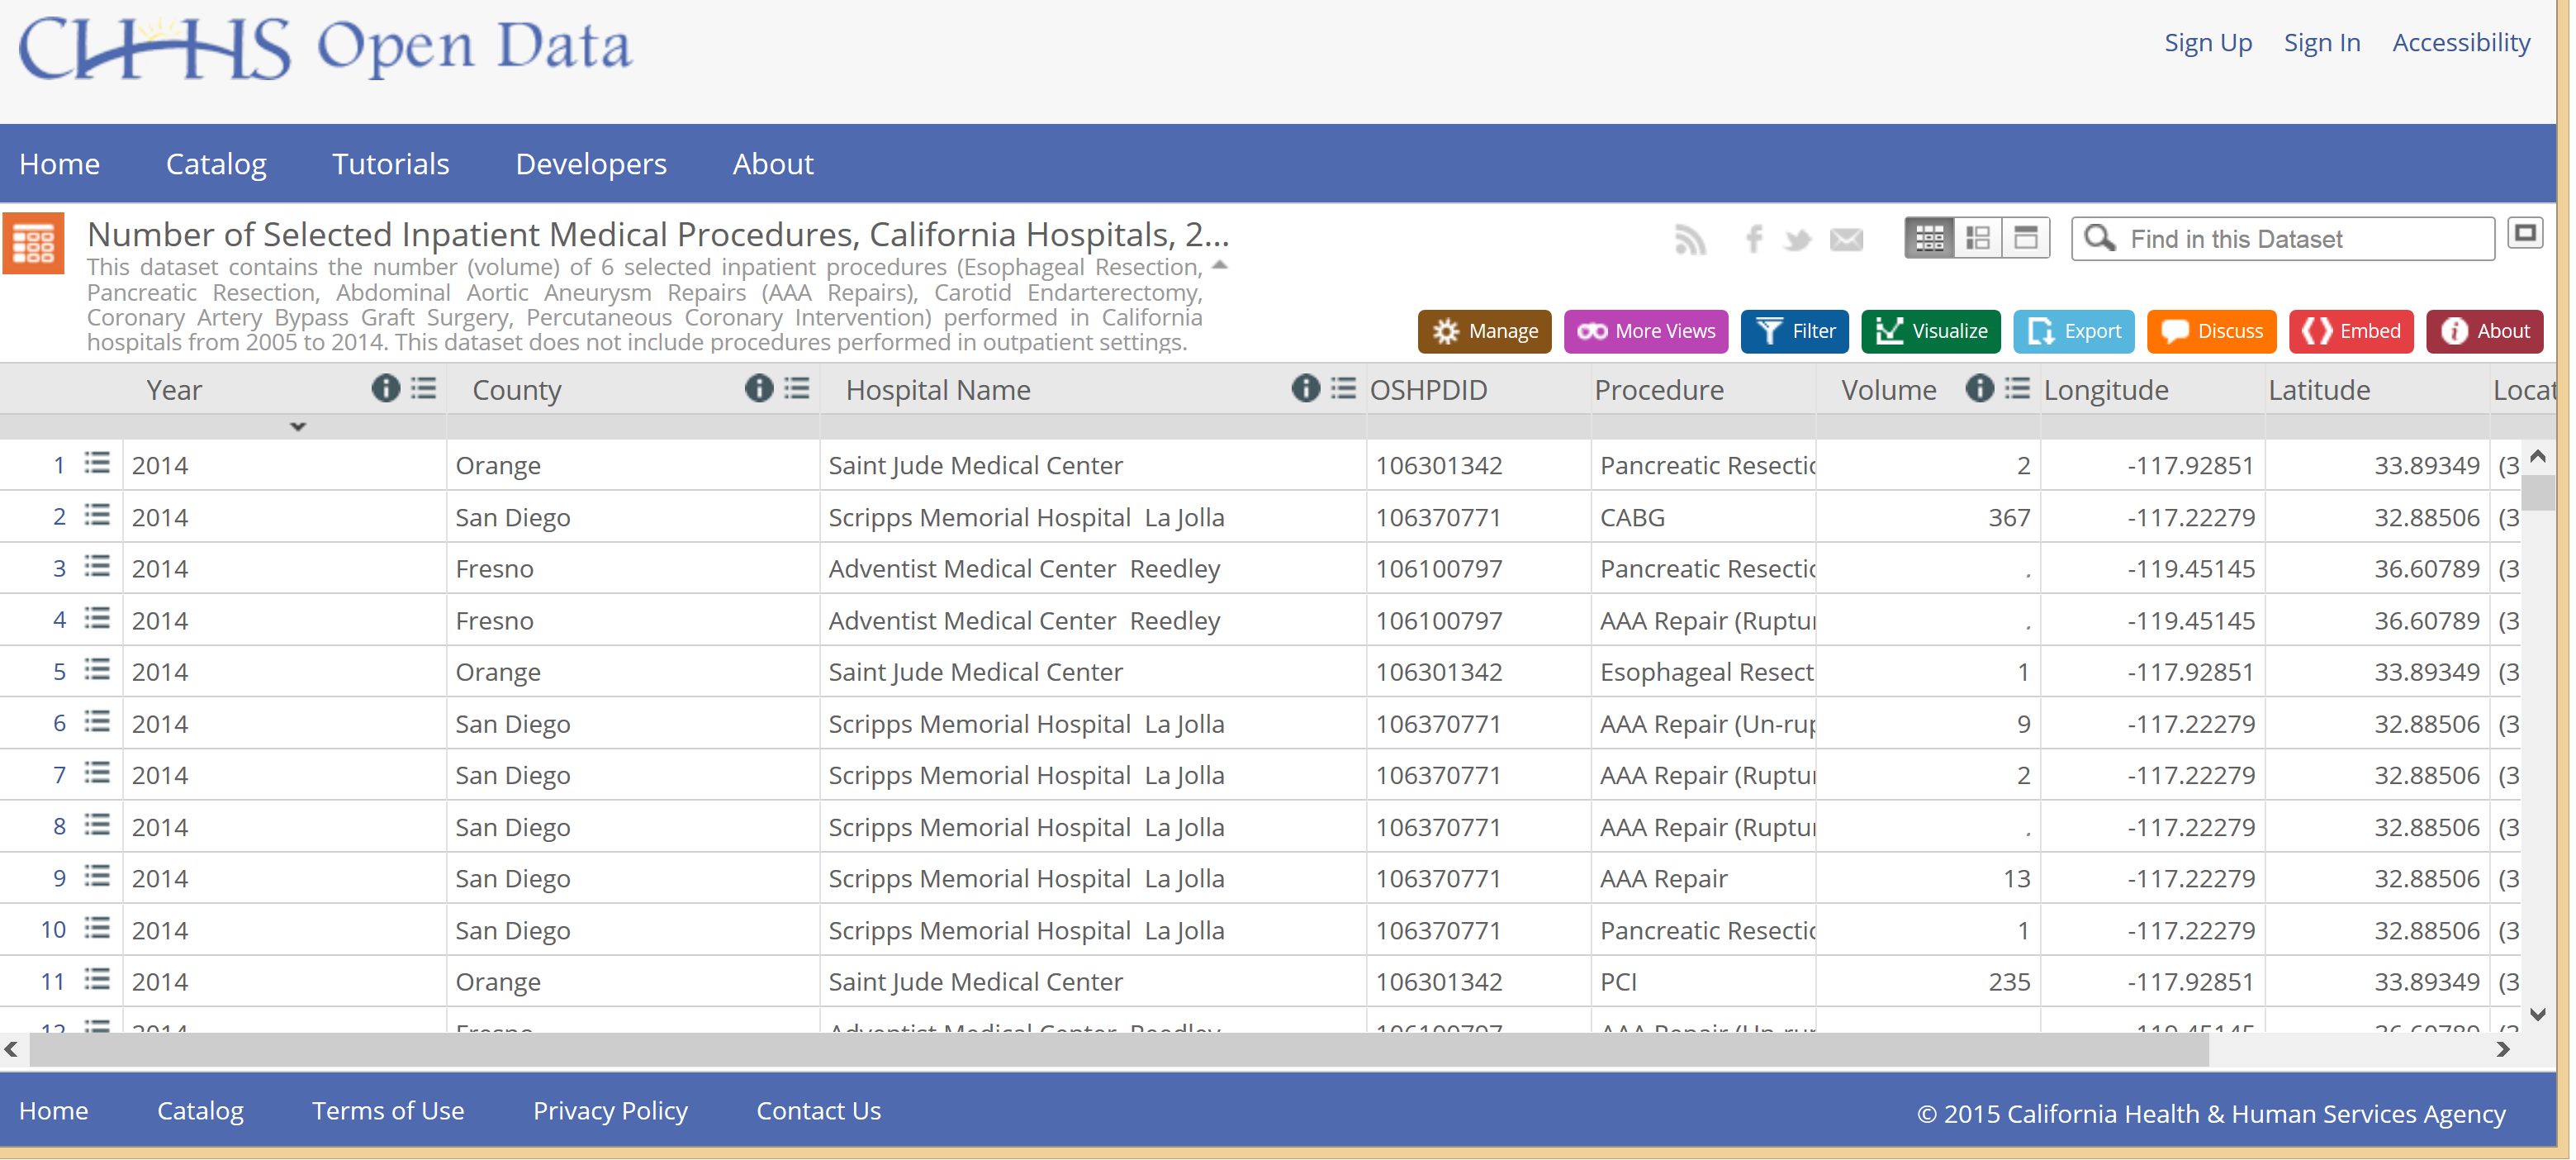
\includegraphics[width=0.7\textwidth]{images/data.png}
    \end{center}  

\newpage   
	\noindent To read it into R, type:
  		\begin{lstlisting}[ basicstyle=\footnotesize ]
df <- read.table(
  "Number_of_Selected_Inpatient_Medical_Procedures__California_Hospitals__2005-2014.csv",
  sep = ",",
  header=TRUE,
  stringsAsFactors = FALSE
  )
    \end{lstlisting}

Check that the file was read-in correctly:
\begin{lstlisting}
dim(df) # 45,438 rows and 9 columns
\end{lstlisting}

Rename the first variable to make it easier to work with:
\begin{lstlisting}
names(df)[1] = 'Year'
		\end{lstlisting}

\end{frame}


% ------------------------------------------------------------
% ------------------------------------------------------------
\section[Summary Plots]{Summary Plots}

\subsection{Scatterplot}
%%%%% New frame
\begin{frame}[allowframebreaks, fragile]
\frametitle{Scatterplot (v0.1)}

To get a quick peak into the numerical variables in the data \ttfamily scatterplotMatrix(): \normalfont
  		\begin{lstlisting}[ basicstyle=\footnotesize ]
# Load package `car' to use scatterplotMatrix():	
library(car)	
scatterplotMatrix(
  x = df[, c("Latitude", "Longitude", "Volume")], 
  smoother = FALSE, 
  reg.line = FALSE
  )
		\end{lstlisting}
% col=rgb(0.4, 0.2, 0.2, alpha=0.5)

        \begin{center}
         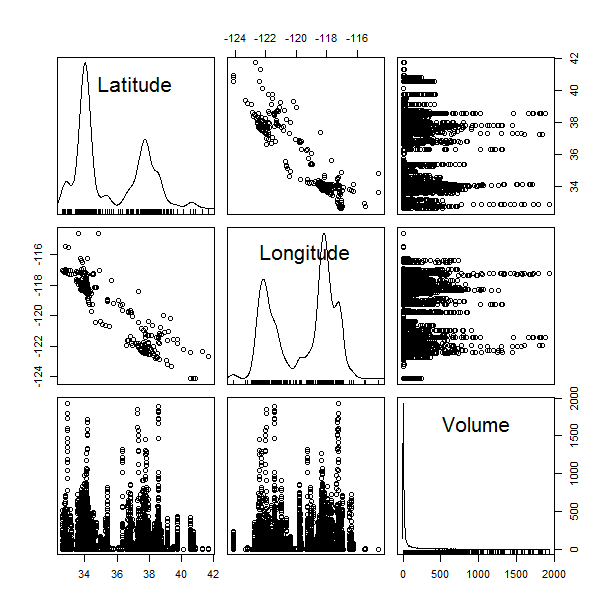
\includegraphics[width=0.63\textwidth]{images/scatterPlot_v0.png}
        \end{center}
\end{frame}

\begin{frame}[allowframebreaks, fragile]
\frametitle{Scatterplot (v0.2)}

To get a quick peak into the numerical variables and the trends in the data, modify arguments of \ttfamily scatterplotMatrix(): \normalfont
  		\begin{lstlisting}[ basicstyle=\footnotesize ]
?scatterplotMatrix # for documentation
library(car)		
scatterplotMatrix(
  x = df[, c("Latitude", "Longitude", "Volume")], 
  reg.line = FALSE
  )
		\end{lstlisting}

        \begin{center}
         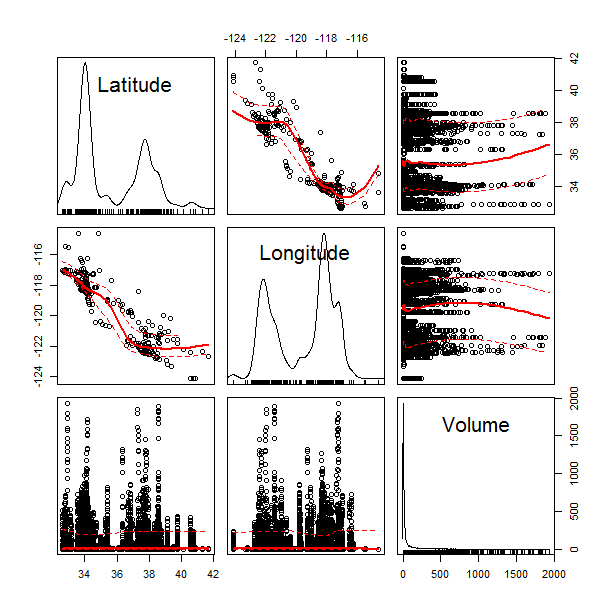
\includegraphics[width=0.63\textwidth]{images/scatterPlot_v1.png}
        \end{center}
\end{frame}

\begin{frame}[allowframebreaks, fragile]
\frametitle{Scatterplot (v0.3)}

To improve the color scheme, modify arguments of \ttfamily scatterplotMatrix().  
  		\begin{lstlisting}[ basicstyle=\footnotesize]
library(car)		
scatterplotMatrix(
  x = df[, c("Latitude", "Longitude", "Volume")], 
  reg.line = FALSE,
  col=c(3,
    "orangered",
    rgb(176/256, 196/256, 222/256, alpha=0.5)
    ), 
  pch=19,
  lwd=3
  )
		\end{lstlisting}
\normalfont
\framebreak
You can specify a color in R via: 
\begin{itemize}
	\item Number (e.g. 1 = black, 2 = red, etc.)
	\item Name (e.g. "black", "red", "dodgerblue")
	\item RGB (e.g. c(0,0,0) = black, c(1,0,0) = red, etc.)
	\item Please see \url{http://research.stowers-institute.org/efg/R/Color/Chart/} for color references. 
\end{itemize}

\noindent Note the order of color arguments. \normalfont
        \begin{center}
         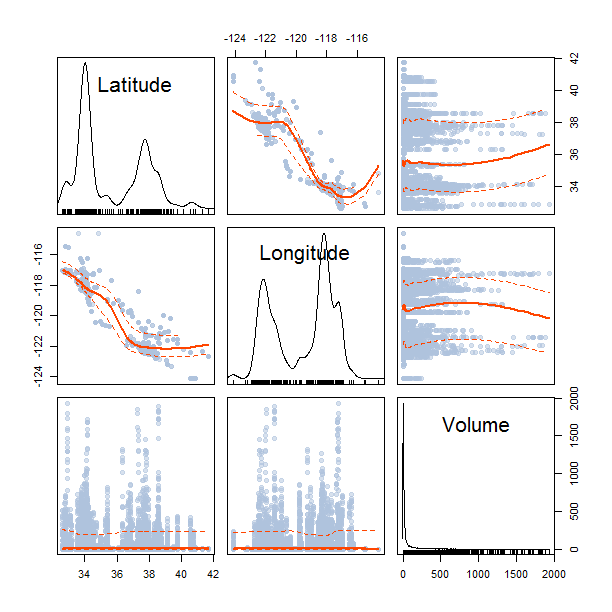
\includegraphics[width=0.63\textwidth]{images/scatterPlot_v3.png}
        \end{center}
\end{frame}

% %---
% \begin{frame}[allowframebreaks, fragile]
% \frametitle{Scatterplot (v0.4)}
%   \framesubtitle{Data = Fiji Earthquakes Since 1964}

% Another way to get a quick peak into the numerical variables in the data is via \ttfamily ggpairs(): \normalfont
%   		\begin{lstlisting}[ basicstyle=\small ]
% library(ggplot2)
% library(GGally)
% ggpairs(
% 	data[, c("Latitude", "Longitude", "Volume")]
% 	)
% 		\end{lstlisting}
% % col=rgb(0.4, 0.2, 0.2, alpha=0.5)

%         \begin{center}
%          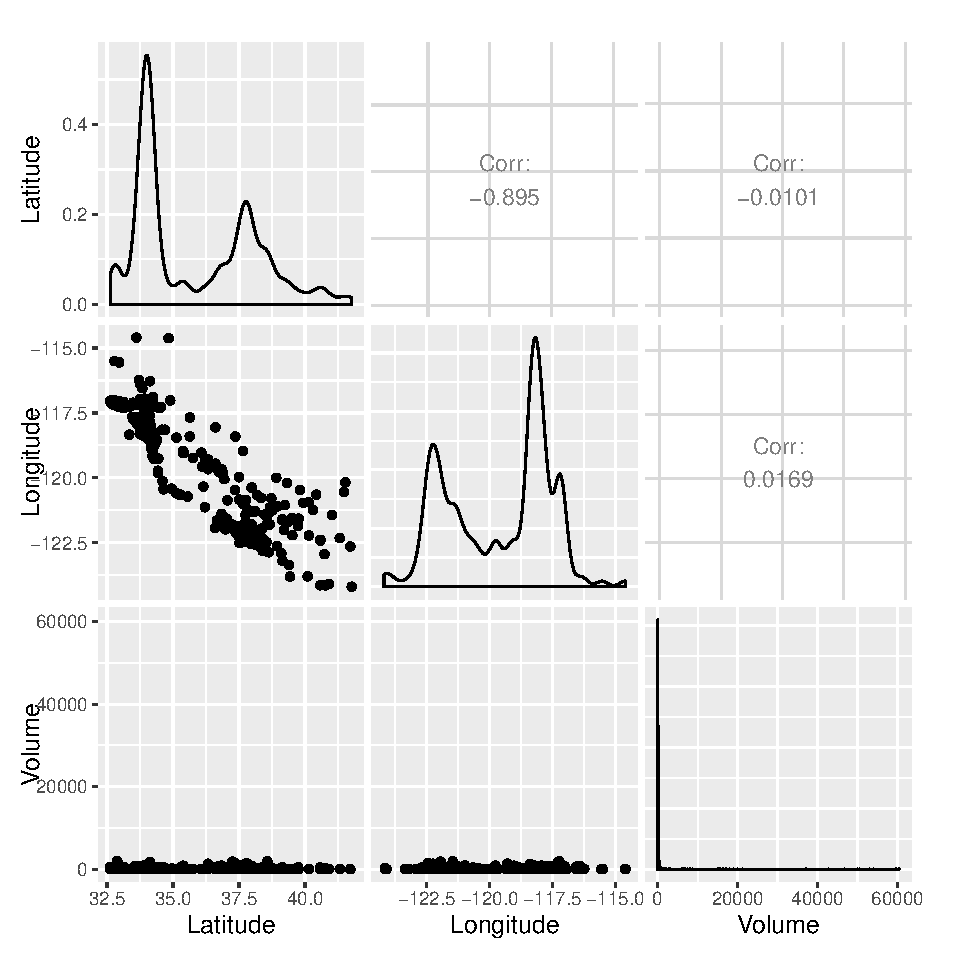
\includegraphics[width=0.6\textwidth]{images/scatterPlot_v4.pdf}
%         \end{center}
% \end{frame}

%%%%% New frame
\subsection{Histogram}

\begin{frame}[fragile, allowframebreaks]
	\frametitle{Histogram}
To see the distribution of one variable, use \ttfamily hist(): \normalfont

    \begin{columns}
      \column{0.40\textwidth}
  \begin{lstlisting}
hist(
  df$Volume, 
  breaks=1000
  )
# Is anything `off'?
  \end{lstlisting}

     \column{0.60\textwidth}
        \begin{center}
           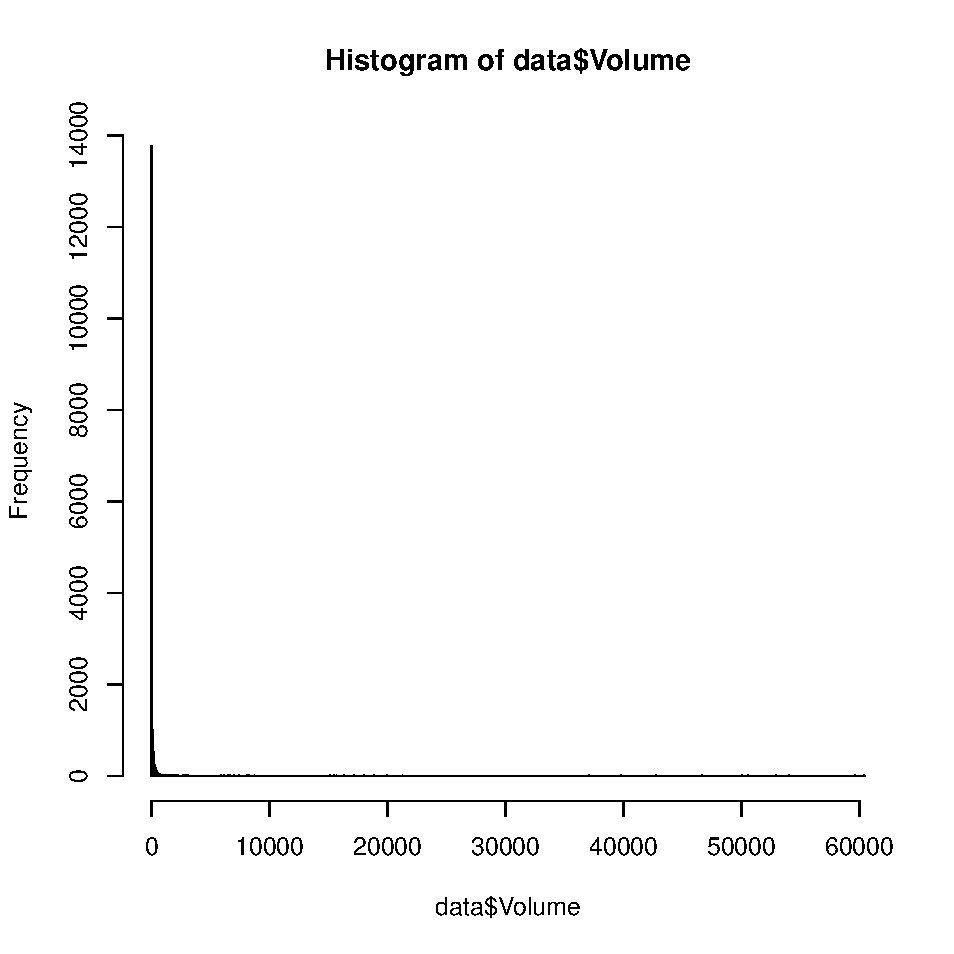
\includegraphics[scale=0.3]{images/histogram.pdf}
        \end{center}  
\end{columns}

\newpage      

Let's examine the potential outlier:
  \begin{lstlisting}
subset(
  x = df, 
  Volume == max(Volume, na.rm=TRUE)
  )
  \end{lstlisting}
{ \tiny
\begin{verbatim}
      ï..Year    County Hospital.Name OSHPDID Procedure Volume Longitude Latitude Location
41783    2005 STATEWIDE     STATEWIDE      NA       PCI  60418        NA       NA         
\end{verbatim}
}

\newpage

Entry seems to be an aggregate number, not county/year level.  To remove the outlier:

    \begin{columns}
      \column{0.50\textwidth}
  \begin{lstlisting}[ basicstyle=\footnotesize]
data_clean <- subset(
  x = df, 
  County != "STATEWIDE"
  )
hist(data_clean$Volume)
# Is anything `off' now? (Exercise.)
  \end{lstlisting}

     \column{0.50\textwidth}
    \begin{center}
       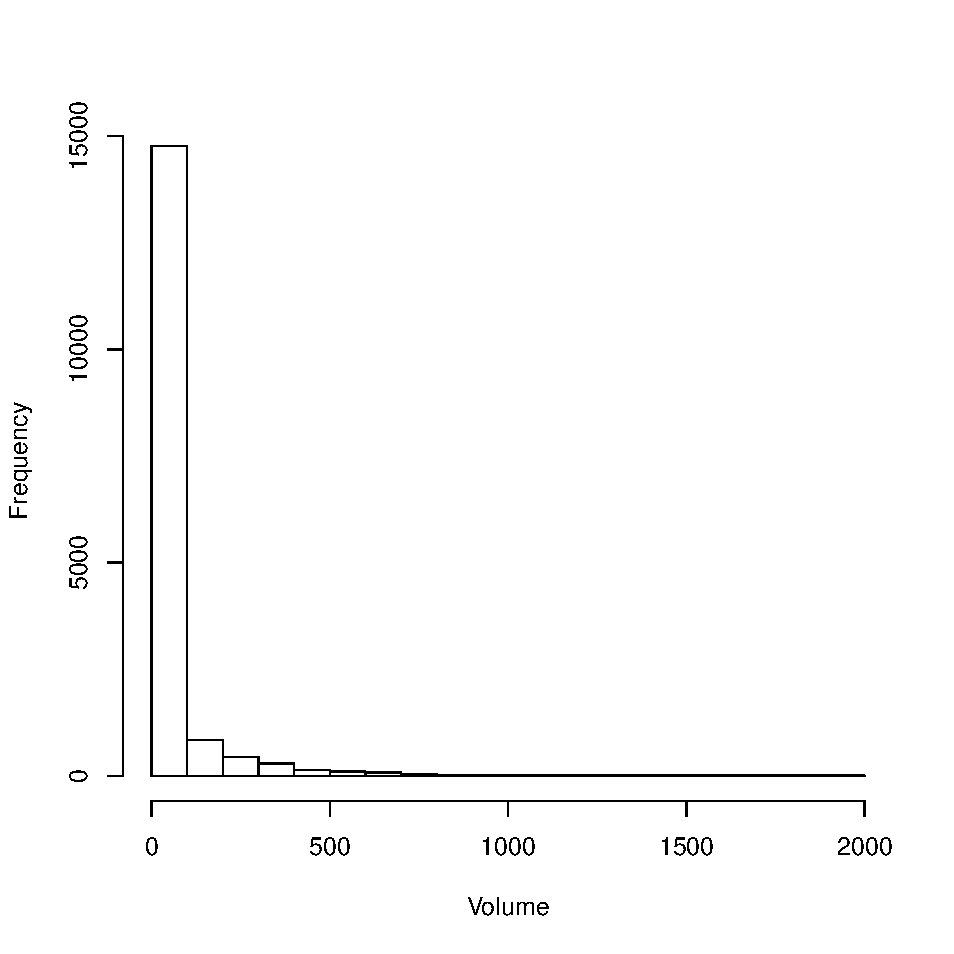
\includegraphics[scale=0.3]{images/histogram2.pdf}
    \end{center}   
\end{columns}

\end{frame}

%----
\begin{frame}[fragile, allowframebreaks]
	\frametitle{'Nicer' Histogram}

To compare two variables side-by-side, use \ttfamily beanplot(): \normalfont

	\begin{lstlisting}[ basicstyle=\footnotesize ]
library(beanplot)
# Subset the data to LA and SF:
data_LA_SF <- subset(
  x = data_clean, 
  County %in% c("Los Angeles", "San Francisco") 
  )

# Orient y-axis labels to be more readable:
op <- par(las=2)
beanplot(
  Volume ~ as.factor(County), 
  data = data_LA_SF, 
  xlab = "",
  log = "y",
  side = "both", 
  col = list( c( grey(0.5), "white"), grey(0.8) ), 
  border = NA, 
  overallline = "median", 
  ll = 0.005,
  show.names=FALSE
  )

legend(
  x = "bottomleft",
  fill=c( grey(0.5), grey(0.8) ), 
  legend=c( "LA", "SF" )
  )
par(op)
	\end{lstlisting}

\newpage
        \begin{center}
	         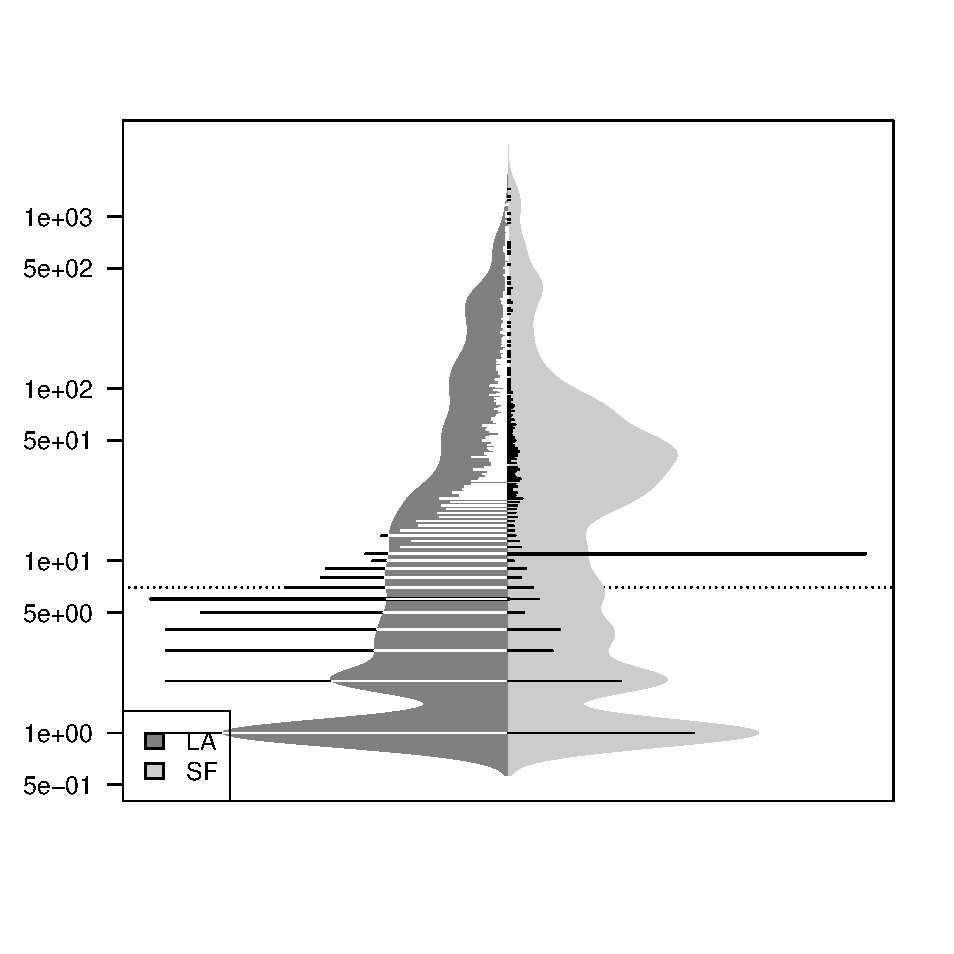
\includegraphics[width=0.65\textwidth]{images/beanplot.pdf}
        \end{center}

\end{frame}

% ------------------------------------------------------------
% ------------------------------------------------------------

% Exercise: compare distributions of Iris data
% ID outlier in dataset

\subsection{Exercise I}
\begin{frame}
	\frametitle{Exercise I}
	In the healthcare data set, after we removed statewide patient admissions, is the largest volume of patients now seen at a Californian hospital a potential outlier?  How do you know?
\end{frame}